\documentclass{report}

\usepackage[utf8]{inputenc}
\usepackage[T1]{fontenc}
\usepackage[french]{babel}
\usepackage{amsmath}
\usepackage{stmaryrd}
\usepackage{fullpage}
\usepackage{microtype}

\usepackage[hidelinks]{hyperref}
\usepackage{pdfpages}

\begin{document}

\section*{Question 1}

\paragraph{} Le gain apporté par le responsable marketing de
\textit{BrainStuffing} pour ce carnet de commande sera de $g(7) + g(0) = 75 +
25 = 100$.

\section*{Question 2}

\paragraph{} $\forall t, 0 \leq t \leq T, m(0, t) = 0$

\section*{Question 3}

\paragraph{}

\begin{align*}
	\forall k \in \llbracket 1, K\rrbracket, \forall t \in \llbracket 0, T \rrbracket,
		m(k, t) = & \max(m(k-1, t-d(k))+g(k), m(k-1, t))) && \text{si} && d(k) \leq t\\
		          & m(k-1, t)                              && \text{sinon} && \\
\end{align*}

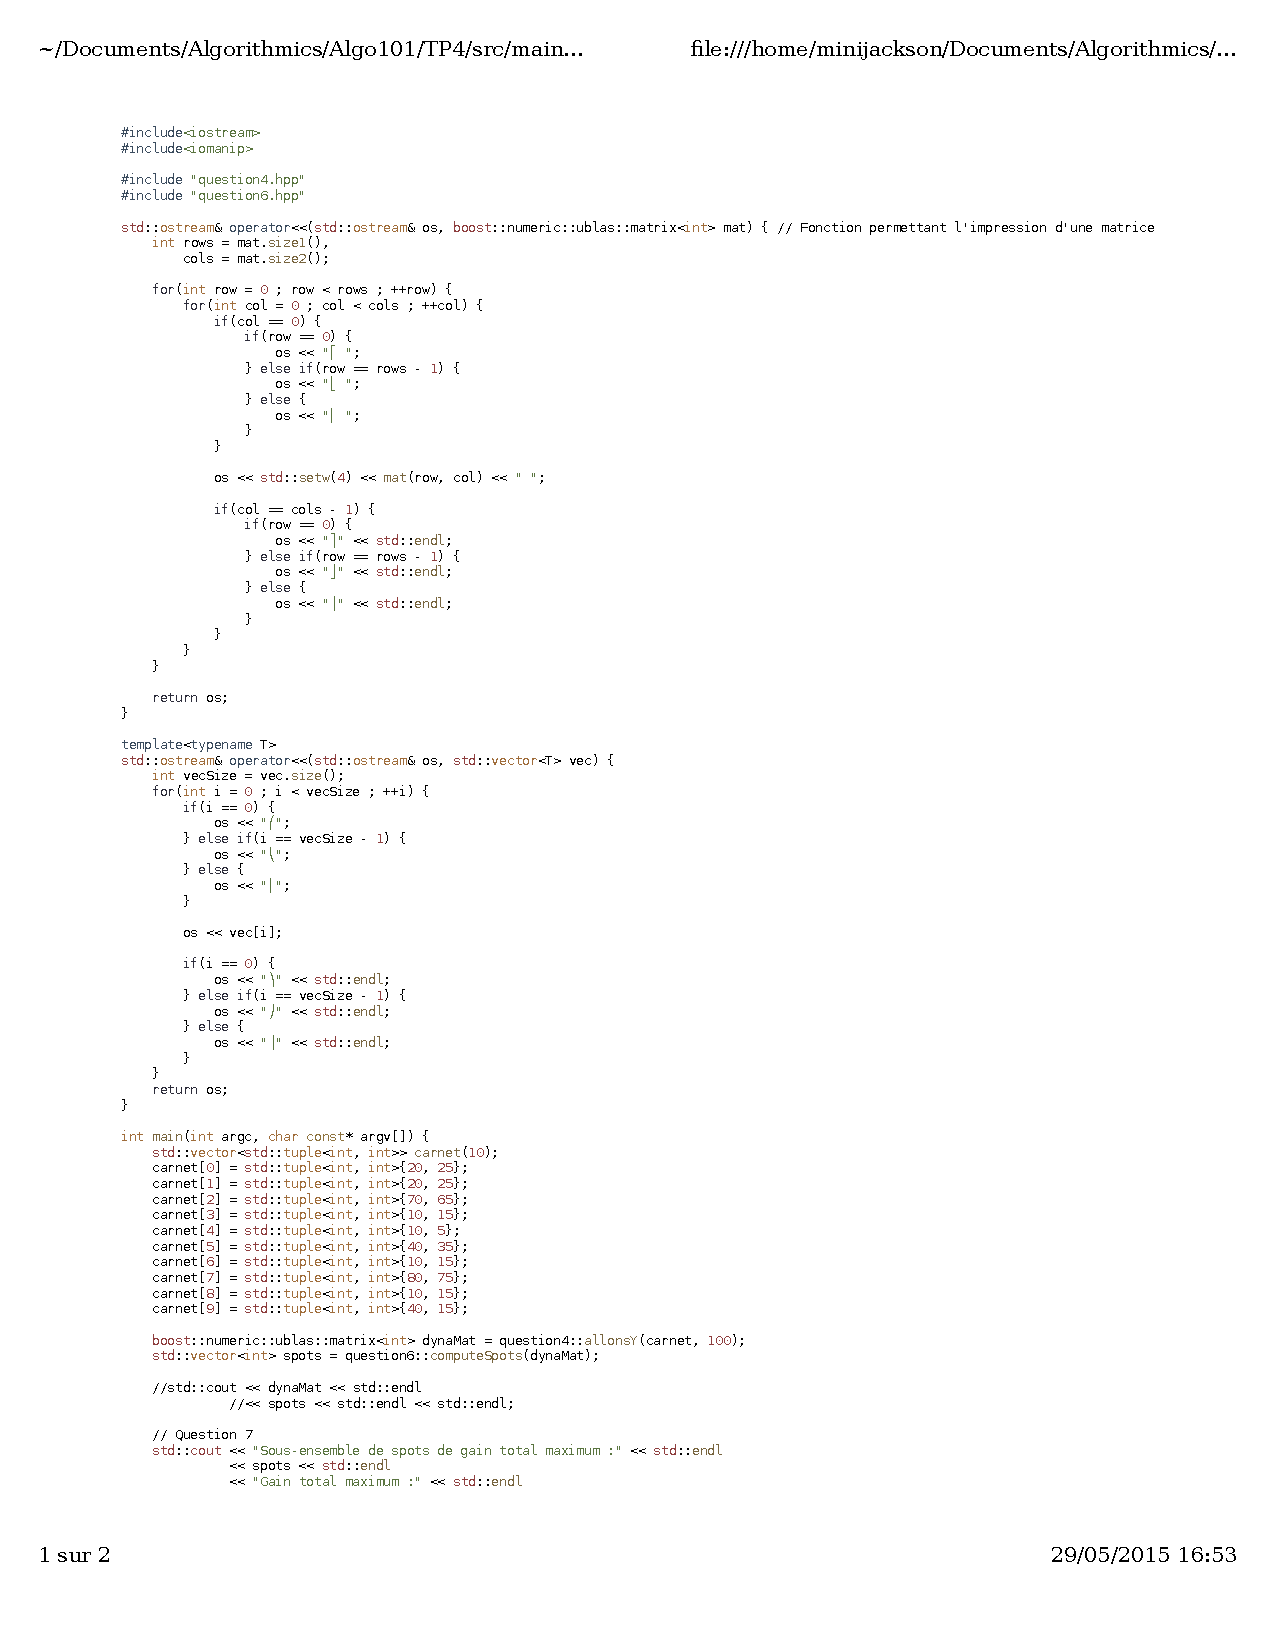
\includepdf{maincpp.pdf}
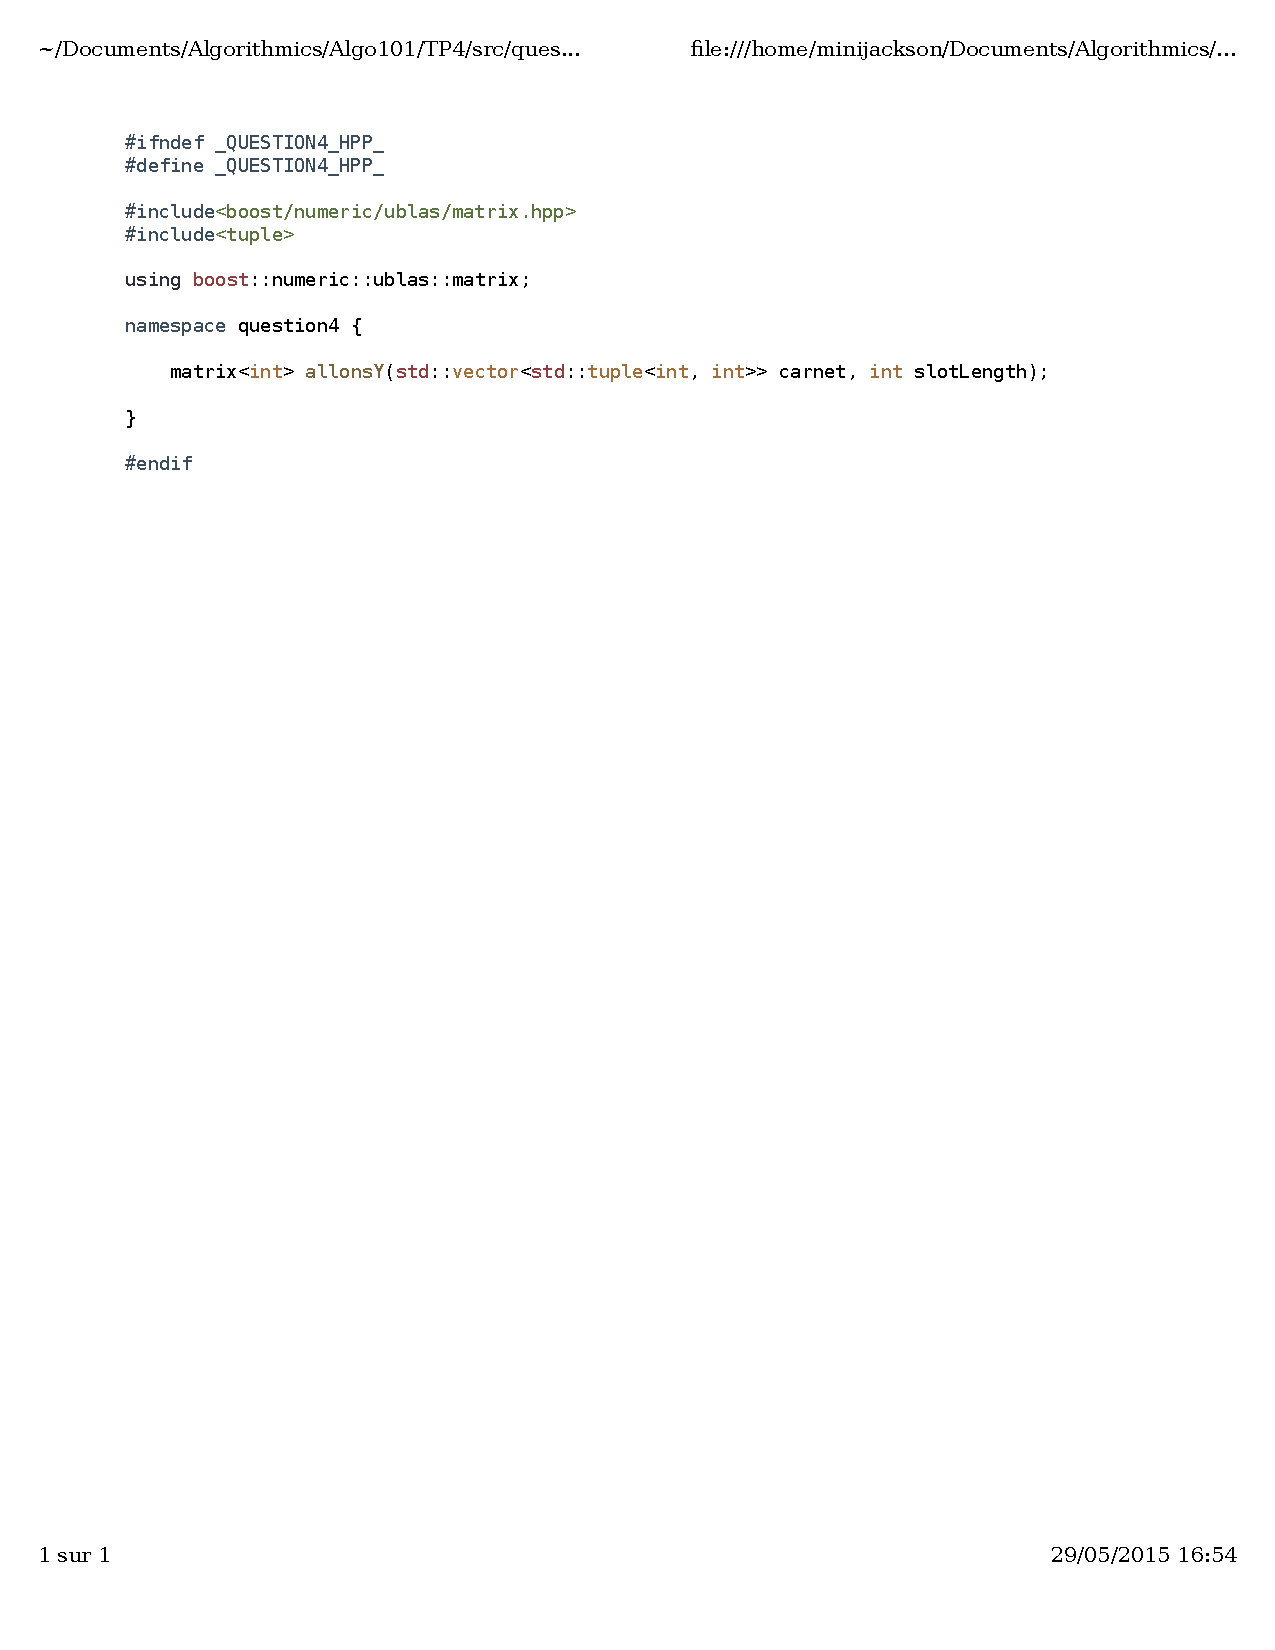
\includepdf{question4hpp.pdf}
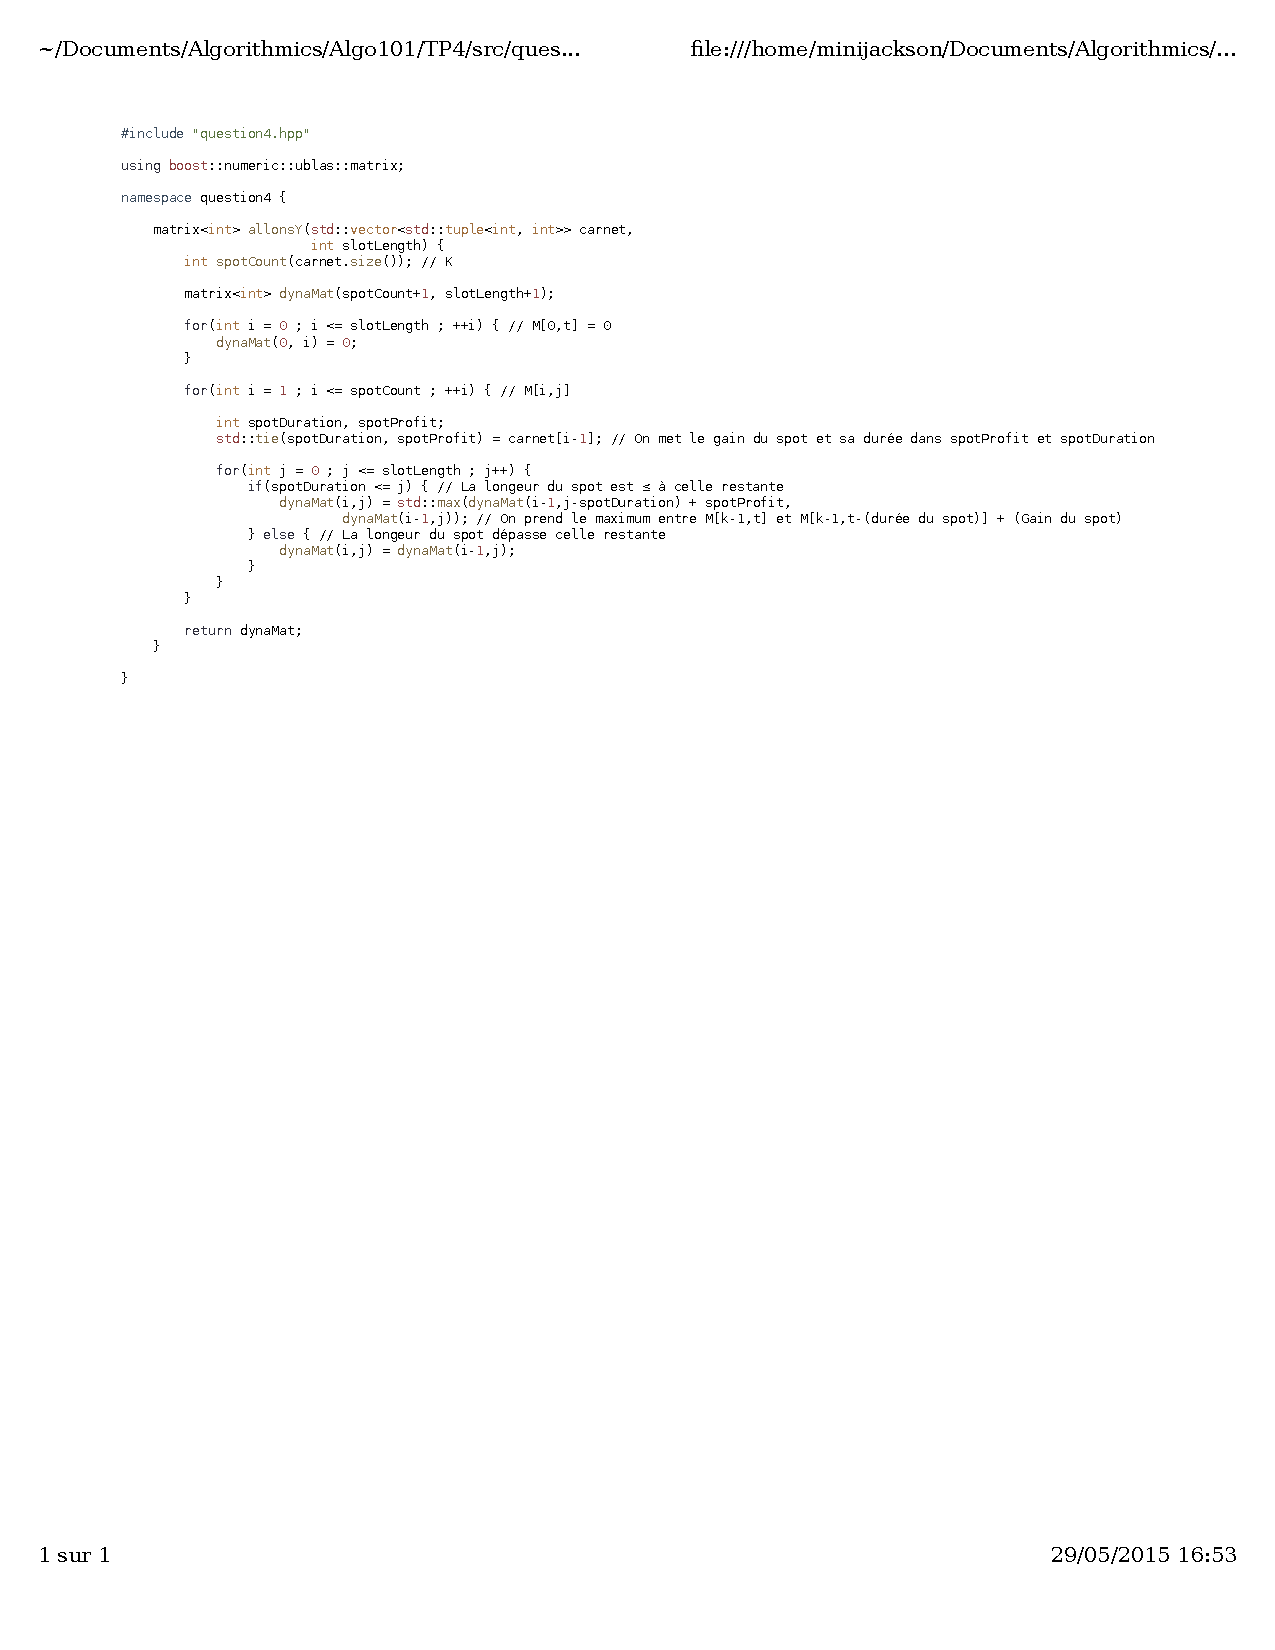
\includepdf{question4cpp.pdf}
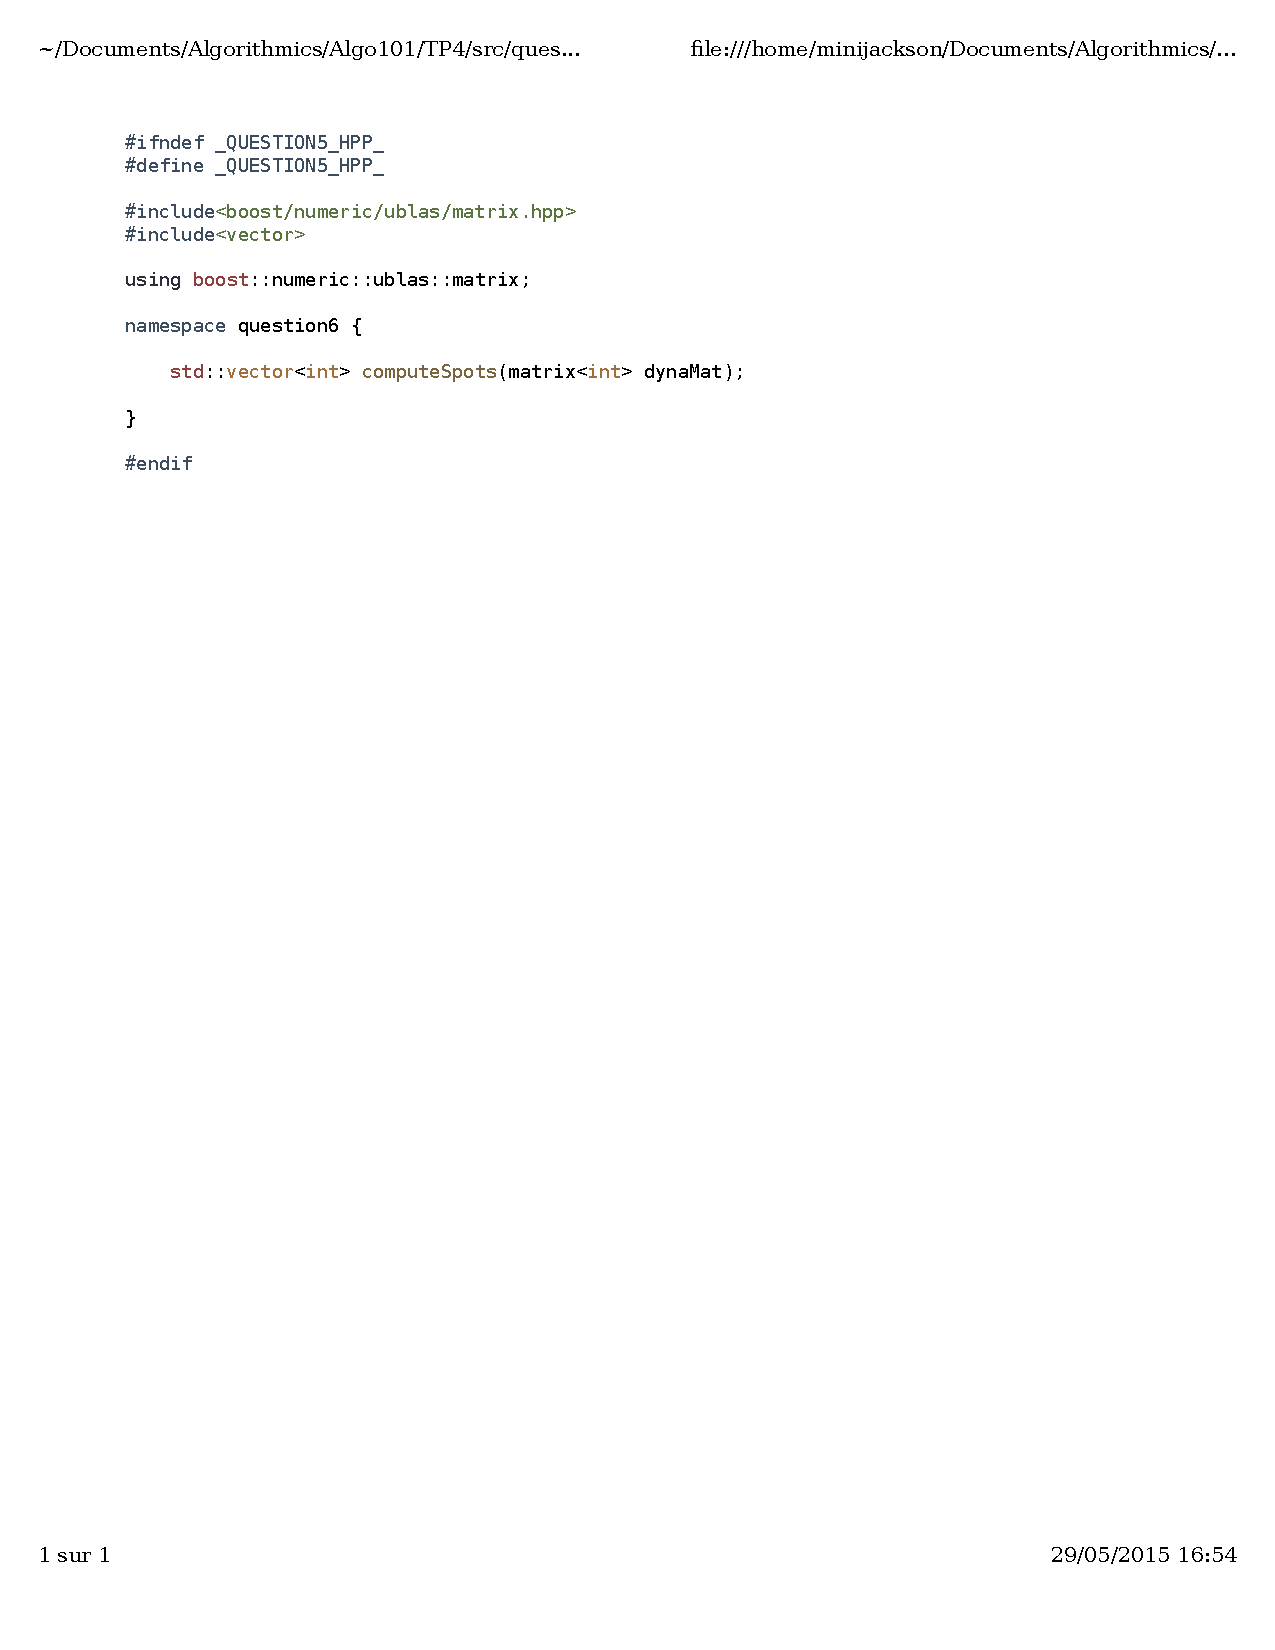
\includepdf{question6hpp.pdf}
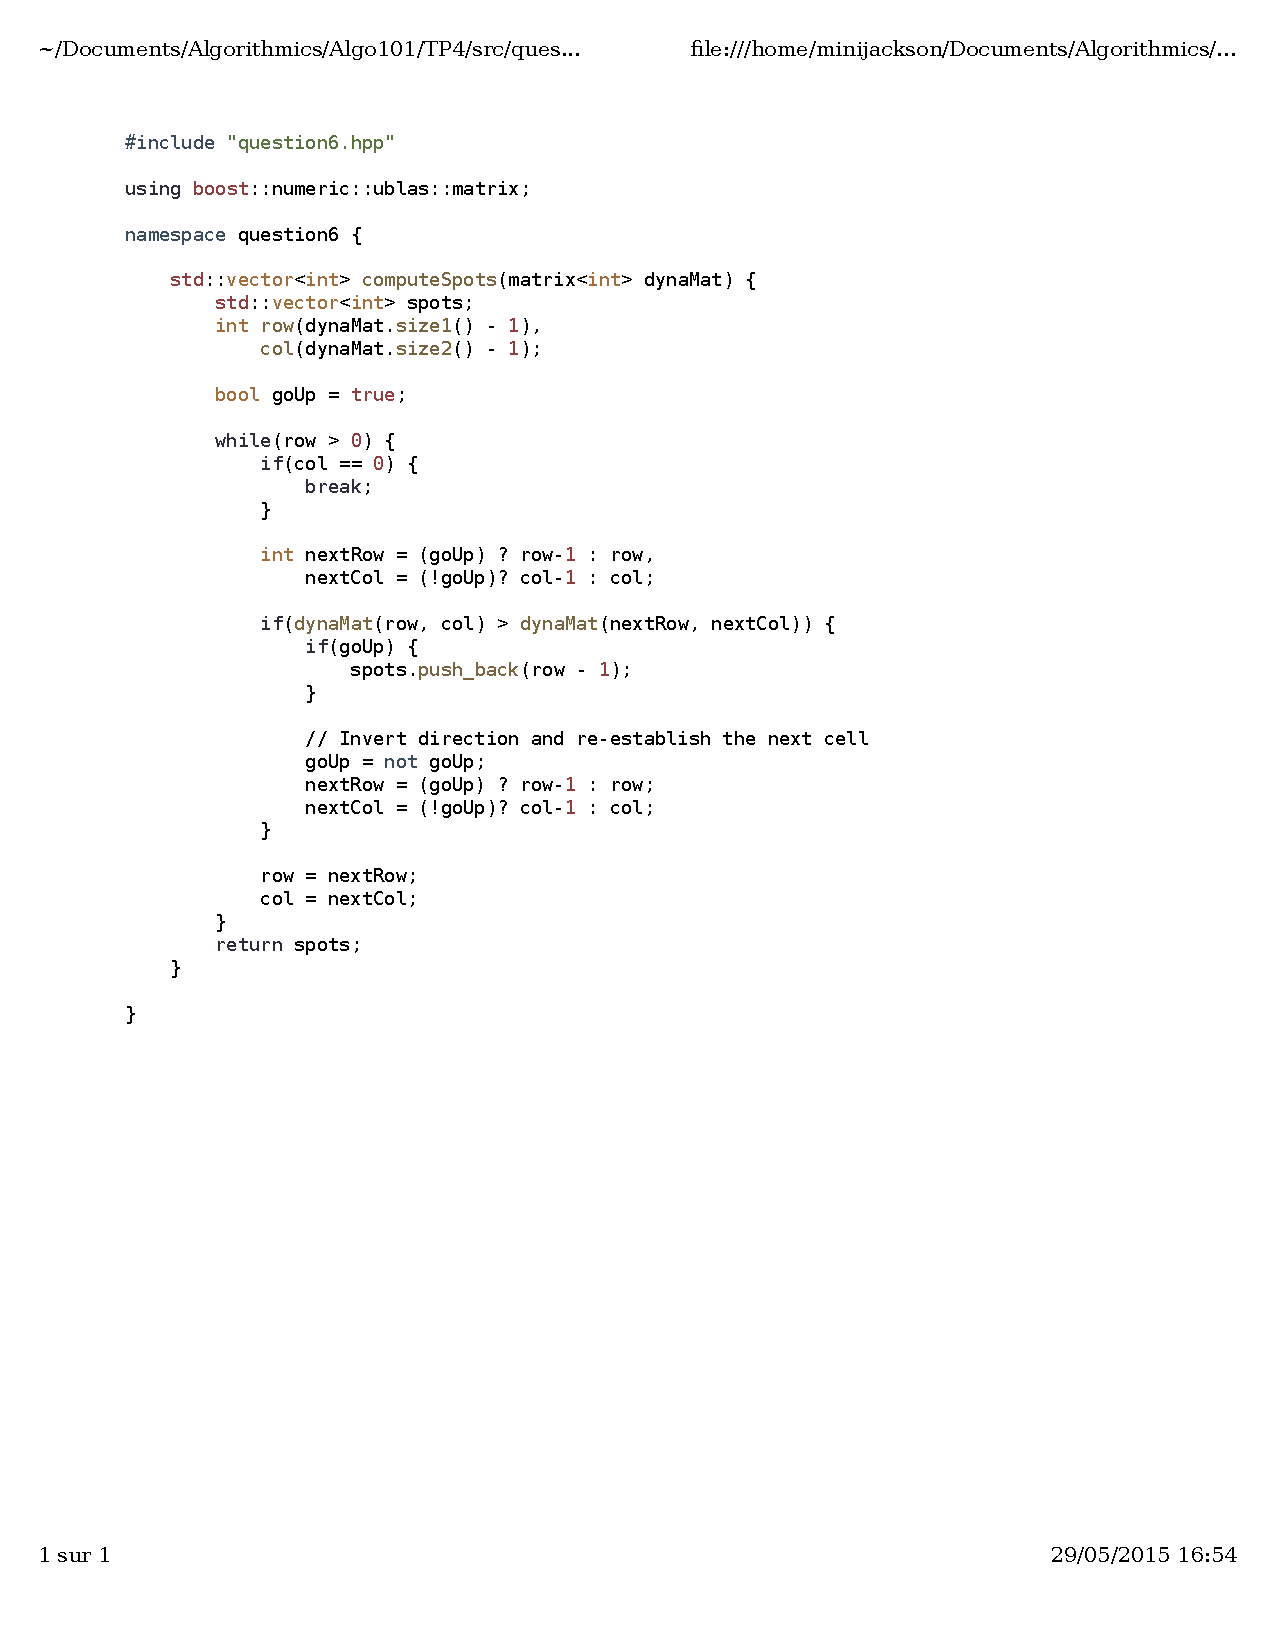
\includepdf{question6cpp.pdf}

\end{document}
